
    Прежде чем исследовать характеры, обсудим сперва саму структуру группоида\footnote{здесь и далее под группоидами подразумеваются связные группоиды}.

    \begin{definition}\cite{MacLane}
        \emph{Группоидом} назывется категория, любая стрелка которой обратима.
    \end{definition}

    \begin{figure}[h]
        \centering
        \[\xymatrix{
            b \ar@(u,l)[]_{\hom(b,b)} \ar[ddrr]^{\hom(b,c)}                     & &                             \\
                                                                                & &                             \\
            a \ar@(l,d)[]_{\hom(a,a)} \ar[uu]^{\hom(a,b)} \ar[rr]_{\hom(a,c)}   & & c \ar@(r,d)[]^{\hom(c,c)}
        }\]
        \caption{группоид}
        \label{cd_groupoid}
    \end{figure}

    Попытаемся найти в группоиде ``что-то вроде базиса''. В некотором 
    группоиде $\Gamma$ выберем произвольную вершину $a$ и рассмотрим её группу 
    петель $G$ и \emph{веер стрелок} $(e, f, g,\ldots)$.

    \begin{definition}
        \emph{Веером стрелок} вершины $a$ группоида $\Gamma$ назовем 
        множество стрелок 
        $V = \{e = \id_a : a \to a,\: f: a \to b,\: g: a \to b,\: \ldots\}$, 
        исходящих из вершины $a$ по одной в каждую из вершин группоида, причем 
        $e : a \to a$ есть тождественная стрелка.
    \end{definition}

    \begin{figure}[h]
        \centering
        \[\xymatrix{
            b                                                                           & &     \\
                                                                                        & &     \\
            a \ar@(l,d)[]_{\textstyle e} \ar[uu]^{\textstyle f} \ar[rr]_{\textstyle g}  & & c
        }\]
        \caption{веер}
        \label{cd_groupnfan}
    \end{figure}

    Возникает вопрос: как соотносятся с выделенным ``базисом'' остальные 
    стрелки группоида? Ответ на него дает следующая простая лемма.

    \begin{lemma}\label{lm_1} Для любой стрелки $v : b \to c$ группоида 
        $\Gamma$ существуют, и притом единственные $f,g \in V$ и $h \in G$, 
        такие что
            \begin{equation}\label{arr_represent}
                v = ghf^{-1}.
            \end{equation}
    \end{lemma}
    \begin{proof}
        Действительно, поскольку $v : b \to c$, и $h : a \to a$, стрелки $g$ и 
        $f$ обязаны действовать из $a$ в $c$, и из $a$ в $b$ соответственно, а 
        таковые имеются в $V$ в единственном экземпляре.
        
        Раз теперь известны $v$, $g$ и $f$, существование и единственность 
        стрелки $h \in G$ следует напрямую алгебраически из выражения 
        \eqref{arr_represent}, а именно $h = g^{-1}vf$.
    \end{proof}
    
    Иными словами, мы построили биекцию 
    \begin{equation}\label{iota}
        \iota : \Arr(\Gamma) \to V \times G \times V
    \end{equation}
     --- между стрелками и множеством троек вида $ghf^{-1}$.

    Располагая таким построением, мы опустим кавычки говоря о $(G,V)$ как о 
    \emph{базисе} группоида $\Gamma$, а под \emph{разложением} по этому базису 
    стрелки или множества стрелок с математической точки зрения будем 
    подразумевать образ соответствующего множества при отображении $\iota$.

    Перебирая и фиксируя различные пары $(g,f)$ можно получить разложение 
    группоида по базису $(G, V)$, о чем и говорит
    
    \begin{corollary}\label{cor_repres} (о представлении $\hom$-множеств)
        \begin{itemize}
            \item[a.] $\hom(b,c) = gGf^{-1}$
            \item[b.] $\hom(a,b) = fGe^{-1} = fG$,
            \item[c.] $\hom(b,a) = eGf^{-1} = Gf^{-1}$,
            \item[d.] $\hom(b,b) = fGf^{-1}$, \footnote{Это классическое 
            утверждение об изоморфности всех групп петель в группоиде (которое 
            и позволяет ввести такой объект как фундаментальная группа)}
            \item[e.] $\hom(a,a) = eGe^{-1} = G$,
        \end{itemize}
        где $f : a \to b$, $g : a \to c$, $G = \hom(a,a)$.
    \end{corollary}

    Полезно также отедельно выделить частный случай.

    \begin{definition}
        \emph{Простым группоидом} назовем группоид, фундаментальная группа 
        которого тривиальна.
    \end{definition}

    Для которого, ввиду $G = \{\id_a$\} следствие \ref{cor_repres} принимает вид:

    \begin{corollary}\label{cor_simple_grp}
        В простом группоиде любая стрелка $v : b \to c$, раскладывается в 
        базисе $V$ как
        \[v = gf^{-1},\]
        где $f : a \to b$, $g : a \to c$.
    \end{corollary}
    
    \begin{figure}[h]
        \centering
        \[\xymatrix{
            b \ar@(u,l)[]_{\textstyle fGf^{-1}} \ar[ddrr]^{\textstyle gGf^{-1}}             & &                             \\
                                                                                            & &                             \\
            a \ar@(l,d)[]_{\textstyle G} \ar[uu]^{\textstyle fG} \ar[rr]_{\textstyle gG}    & & c \ar@(r,d)[]^{\textstyle gGg^{-1}}
        }\]
        \caption{фактор-группоид}
        \label{cd_groupoid_repres}
    \end{figure}

    Вернемся к группоиду $\Gamma$ и перерисуем диаграмму \ref{cd_groupoid} с 
    учетом следствия \ref{cor_repres} (рис.~\ref{cd_groupoid_repres}). 
    Диаграмма \ref{cd_groupoid_repres} напоминает некую ``факторизацию'', и 
    действительно, если под стрелками на диаграмме понимать не $\hom$-множества,
    а просто стрелки, то мы получим диаграмму \emph{фактор-группоида} 
    $\Gamma/\Phi_\Gamma$\footnote{Пользуясь стандартным 
    определением факторизации категории\cite{MacLane}, подобно тому как это 
    делается в обыкновенных группах, можно ввести 
    факторизацию группоида по любой нормальной подгруппе фундаментальной 
    группы, в том числе и по ней самой.} по фундаментальной группе $\Phi_\Gamma$, 
    где названия стрелок соответствуют прообразам 
    факторизации. Мы не будем здесь строго вводить понятие фактор-группоида, 
    ибо в нашем случае он предствляет из себя всего-навсего \emph{простой 
    группоид} с тем же набором объектов что и исходный.

    При виде диаграммы \ref{cd_groupoid_repres} кажется само собой разумееющимся
    \begin{statement}[о разложении группоида]\label{st_groupoid_decomp}
        \begin{equation}
            \Gamma \simeq \textstyle{\Gamma / \Phi_\Gamma \times \Phi_\Gamma}.
        \end{equation}
    \end{statement}

    Перед доказательством утверждения \ref{st_groupoid_decomp} напомним тот 
    факт, что \emph{группа является категорией --- частным случаем группоида с одним 
    объектом}, и 
    \begin{definition}\cite{MacLane}
        \emph{Произведением} двух данных категорий $B$ и $C$, называется 
        категория $B \times C$, объекты которой~--- пары $(b,c)$ объектов $b$ из 
        $B$ и $c$ из $C$; стрелки $(b,c) \to (b',c')$~--- пары $(f,g)$ стрелок 
        $f : b \to b'$ и $g : c \to c'$, a композиция двух таких стрелок
        \[(b,c) \stackrel{(f,g)}{\longrightarrow} (b',c') \stackrel{(f',g')}{\longrightarrow} (b'',c'')\]
        определяется в терминах композиции в категориях $B$ и $C$ по формуле
        \[(f',g') \circ (f,g) = (f' \circ f, g' \circ g).\]
    \end{definition}

    \begin{proof}
    
        Построим явно изоморфизм~--- функтор $i : \Gamma \to 
        \Gamma / \Phi_\Gamma \times \Phi_\Gamma$.

        Для этого выделим некоторый базис $(G = \hom(a,a), V\text{~--- веер } a)$ 
        группоида $\Gamma$, и для удобства отождествим $\Phi_\Gamma$ с $G$, а 
        веер вершины $a$ в $\Gamma / \Phi_\Gamma$ с $V$.

        Тогда $i$ зададим следующим образом:
        \begin{itemize}
            \item [на объектах:] $i : d \mapsto (d,\theta)$;
            \item [на стрелках:] $i : v \mapsto (gf^{-1},h)$, где 
            $(g,h,f^{-1}) = \iota(v)$.
        \end{itemize}

        Биективность и функторность $i$ очевидна вследствие определения 
        биекции $\iota$, леммы \ref{lm_1} и ее следствий. Впрочем, в этом также 
        можно наглядно убедится взглянув на схему, 
        изображенную на рис.~\ref{cd_groupoid_iso}.

        \begin{figure}[h]
            \centering
            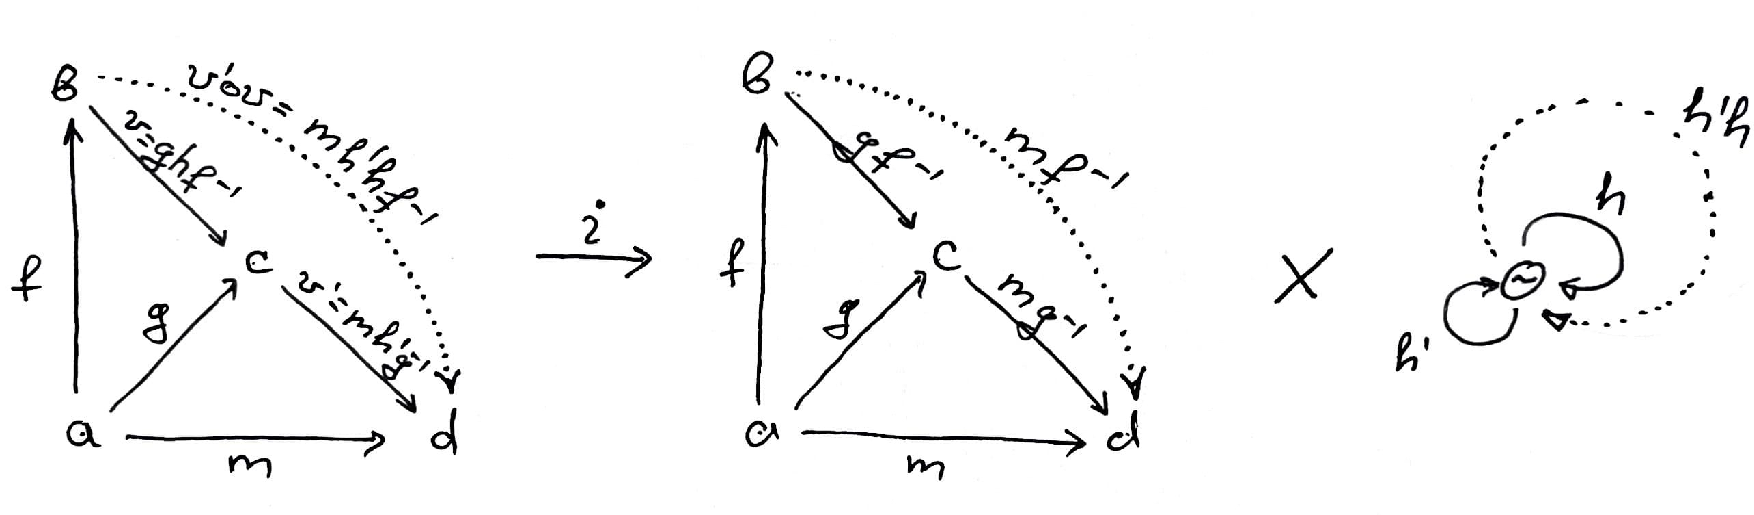
\includegraphics[width=\textwidth]{pictures/cd_grp_iso.pdf}
            \caption{изоморфизм}
            \label{cd_groupoid_iso}
        \end{figure}
    \end{proof}

        Теперь мы готовы перейти к обсуждению характера.